\documentclass[text06.tex]{subfiles}
\begin{document}
\newpage
\section{ヘッドセットの使い方}
\ruby{演習}{えん|しゅう}の前に、ヘッドセットの\ruby{設定}{せっ|てい}をしましょう。ヘッドセットとは、コンピュータなどから音声を出力するためのヘッドフォンと、コンピュータなどに音声を入力するためのマイクが一体型になったものです。\\
まずはラズベリーパイの\ruby{電源}{でん|げん}を入れる前に、ヘッドセットとラズベリーパイをつないでおきます。
ヘッドセットがラズベリーパイに\ruby{接続}{せつ|ぞく}されていると、画面の右上にマイクのアイコンが追加されます。

\begin{figure}[H]
\begin{center}
    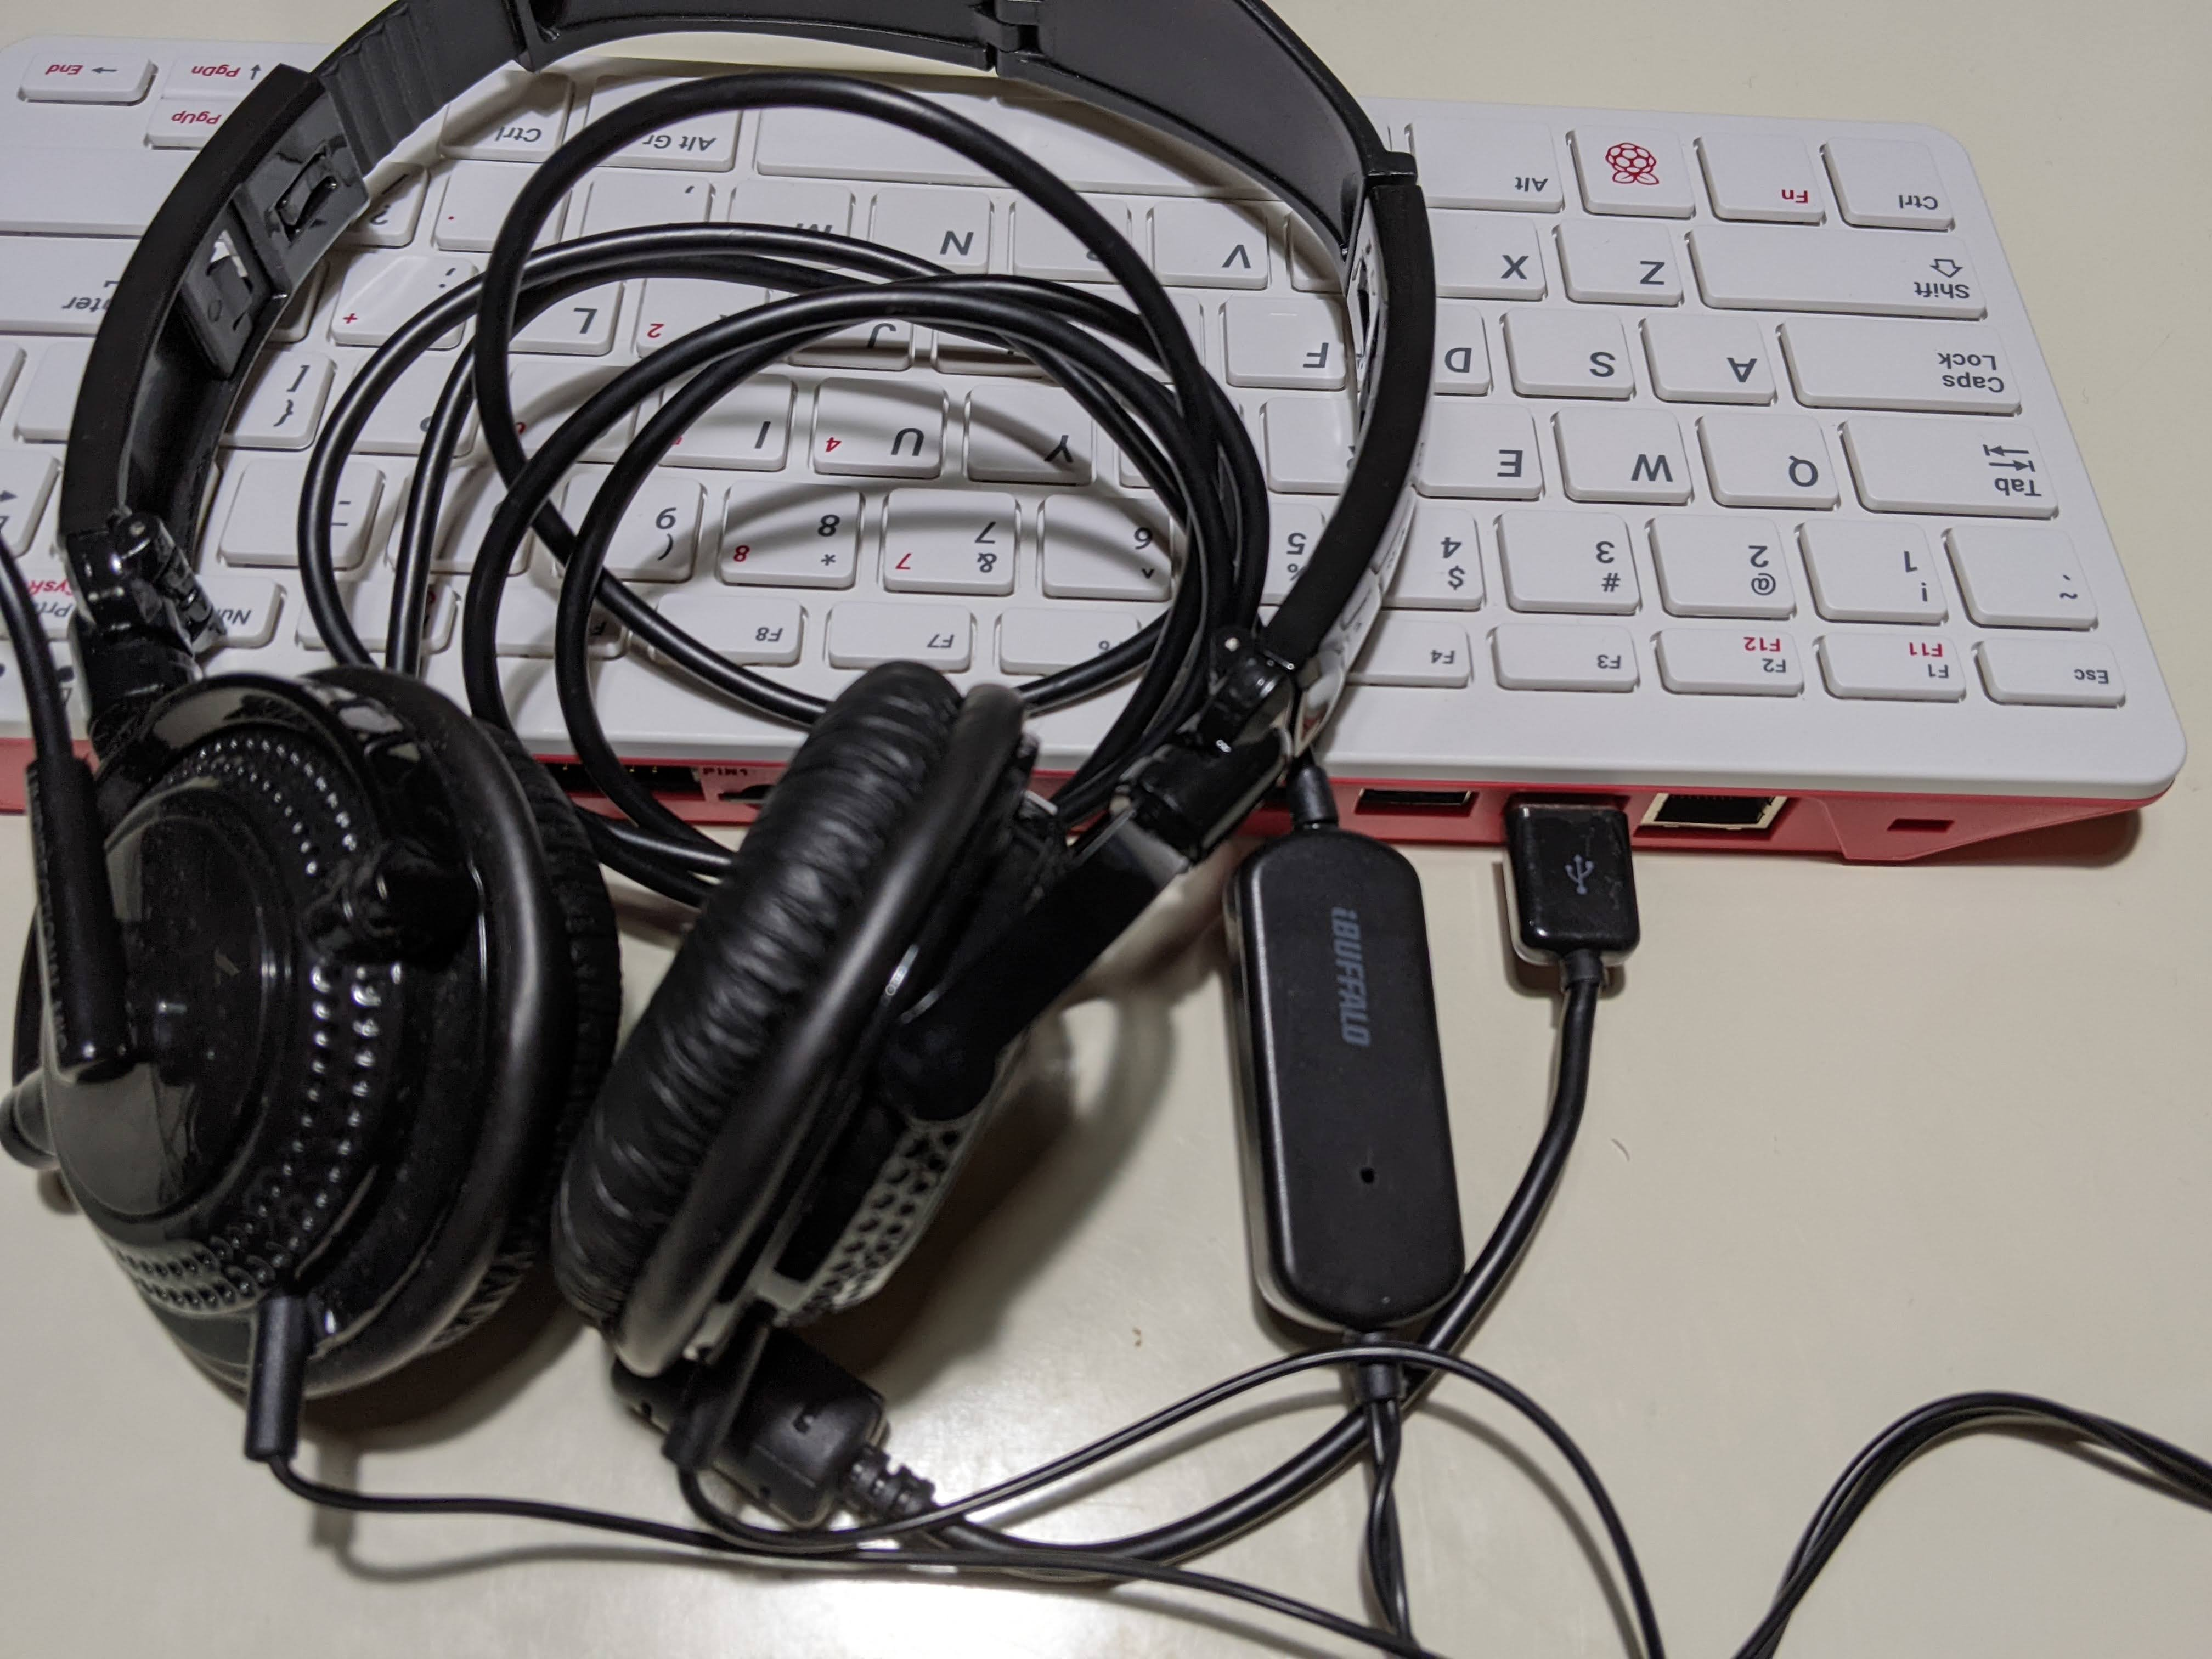
\includegraphics[width=.6\linewidth]{../../asset/image/how_to_connect_headset.jpg}
    \caption{ヘッドセットのつなげかた}
    \label{つなげかた}
\end{center}
\end{figure}

ヘッドセットの出力音量はヘッドセットにつながっているコントローラーか、ディスプレイ右上のスピーカーのアイコンで調整できます。

\begin{figure}[H]
\begin{center}
    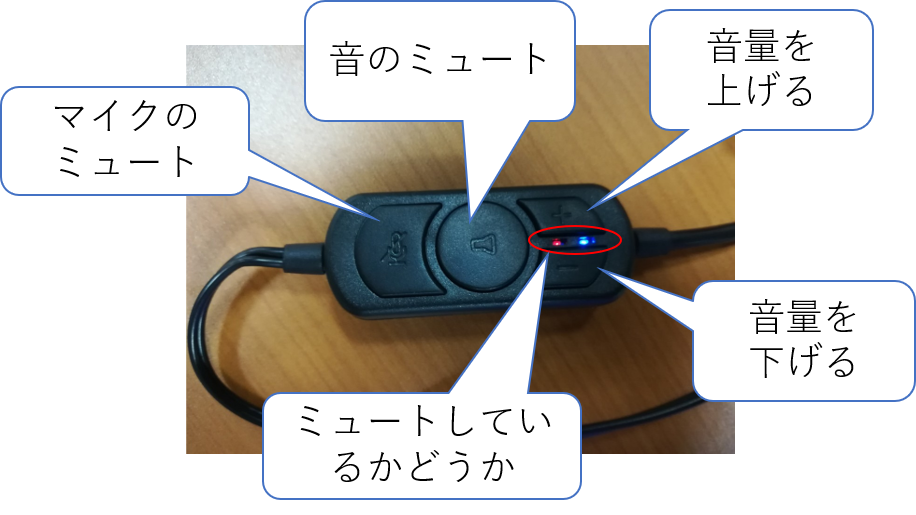
\includegraphics[width=.6\linewidth]{../../asset/image/text06-img004.png}
    \caption{ヘッドセットのコントローラーの使い方}
    \label{ヘッドセットのコントローラーの使い方}
\end{center}
\end{figure}

ヘッドセットのコントローラーの一番左のボタンでマイクのミュートを切りかえることができます。ミュートとは音を消すことです。マイクがミュートしているときは赤色のLEDが光っています。マイクを使うときはミュートを\ruby{解除}{かい|じょ}して、赤色のLEDが光っていないようにしましょう。真ん中のボタンは音のミュートです。音が聞こえないときはここを\ruby{押}{お}してみましょう。右側のボタンは ``+" で音量を上げる、``-" で音量を下げることができます。
ヘッドセットの出力音量はディスプレイの右上にあるスピーカーのアイコンからも設定できます。

次に、音を出す音声デバイスを\ruby{選択}{せん|たく}しましょう。ディスプレイの右上にあるスピーカーアイコンを右クリックしてください。

\begin{minipage}[t]{0.48\linewidth}
    \begin{figure}[H]
        \begin{center}
            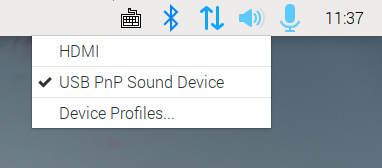
\includegraphics[width=\linewidth]{../../asset/image/select_sink.png}
            \caption{使う音声出力デバイスの選択と設定}
            \label{使う音声デバイスの選択と設定}
        \end{center}
    \end{figure}
\end{minipage}
\begin{minipage}[t]{0.48\linewidth}
    \begin{figure}[H]
        \begin{center}
            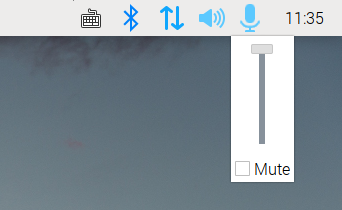
\includegraphics[width=\linewidth]{../../asset/image/microphone_volume.png}
            \caption{マイクの入力音量の調節方法}
            \label{microphone_volume}
        \end{center}
    \end{figure}
\end{minipage}

図 \ref{使う音声デバイスの選択と設定} に使うことのできるデバイスが\ruby{表示}{ひょう|じ}されます。HDMIとはディスプレイのことです。これを左クリックするとディスプレイから音を出すことができます。\aruby{USB}{ユーエスビー} \aruby{PnP}{プラグ・アンド・プレイ} \aruby{Sound}{サウンド} \aruby{Device}{デバイス}は接続したヘッドセットのことです。ヘッドセットを使うときはこちらを左クリックします。
教室ではヘッドセットを使います。おうちでは、ディスプレイやテレビから音声を出力することもできます。

マイクの入力音量を変えるときはマイクのアイコンを左クリックし、表示されたスライドバーを調節します。



教室ではヘッドセットで音を聞き、ヘッドセットのマイクで音声を入力するので、図\ref{使う音声デバイスの選択と設定}のように USB PnP Sound Device を選択し、図\ref{microphone_volume}のようにマイクの入力音量を最大にしておきましょう。


% FIXME: Make a macro and share 05/contents/chap05_02_1.tex for DRY principle.
\begin{itembox}[c]{\Large\textcolor{red}{注意！}}
マイクのアイコンを右クリックしたときに現れるコンテクストメニューの「\aruby{USB}{ユーエスビー} \aruby{PnP}{プラグ・アンド・プレイ} \aruby{Sound}{サウンド} \aruby{Device}{デバイス}」 (図 \ref{pplug-volume_mic_context_menu}) をクリックしないように注意してください。
クリックしてしまうと、一時的にマイクが使用できなくなります。
図 \ref{pplug-volume_mic_context_menu} のように、チェックが外れている状態のときにマイクが使用できます。
\end{itembox}

\begin{figure}[H]
    \begin{center}
      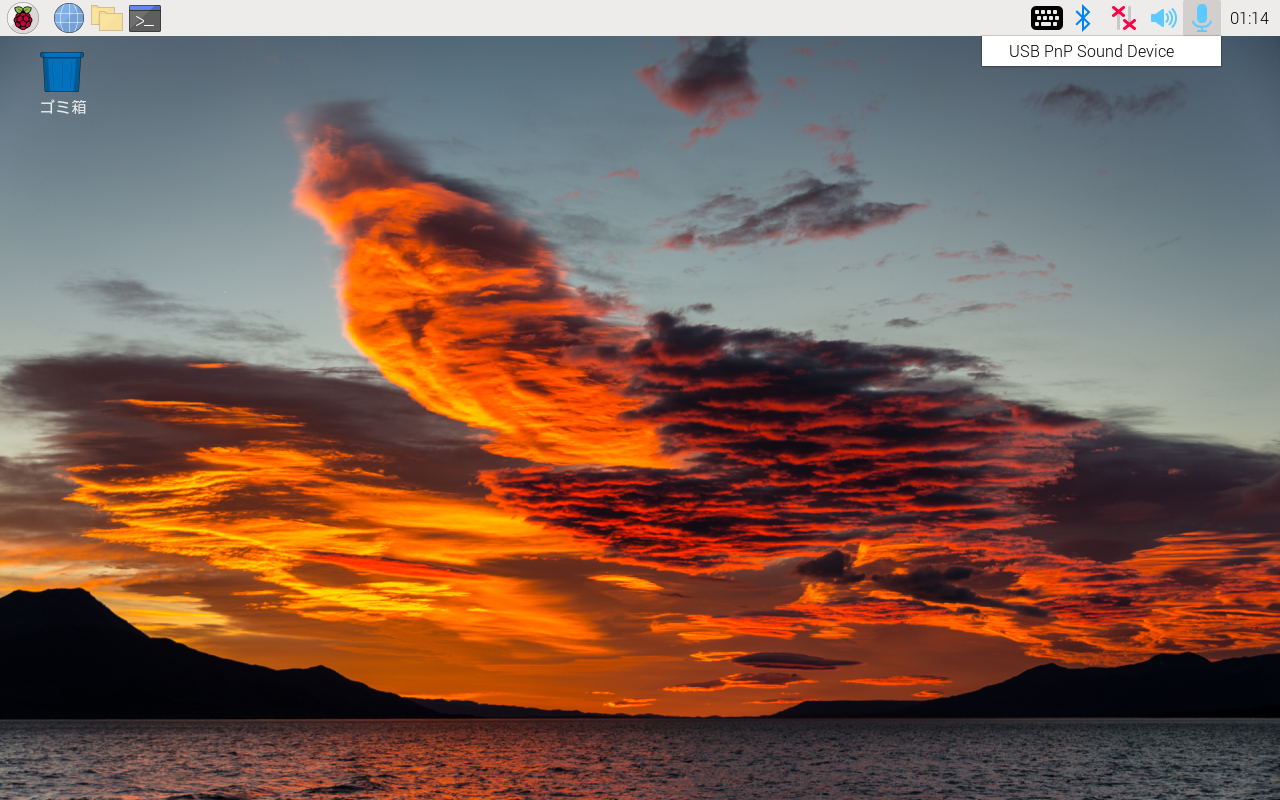
\includegraphics[width=\linewidth]{../../asset/image/pplug-volume_mic_context_menu.png}
      \caption{右上の USB PnP Sound Device はクリックしないよう注意！}
      \label{pplug-volume_mic_context_menu}
    \end{center}
\end{figure}

もしもマイクアイコンのコンテクストメニューで「\aruby{USB}{ユーエスビー} \aruby{PnP}{プラグ・アンド・プレイ} \aruby{Sound}{サウンド} \aruby{Device}{デバイス}」を押してしまい，マイクが使えなくなってしまった場合は、以下の手順に従ってください。
まず、右上のスピーカーアイコンを右クリックし、「デバイスプロファイル…」をクリックしてください (図 \ref{pplug-volume_speaker_context_menu})。
すると図 \ref{pplug-volume_device_profile_dialog_top} のように、新しいウィンドウが現れます。
USB PnP Sound Device の下にあるプルダウンメニューをクリックし、一度「アナログステレオ 出力」をクリックします (図 \ref{pplug-volume_device_profile_dialog_only_output})。
もしはじめから「アナログステレオ 出力」が選択されていた場合は、一度「オフ」をクリックしてからもう一度「アナログステレオ 出力」をクリックしてください。
そのあと「アナログステレオ 出力 + モノ 入力」を選択してください (図 \ref{pplug-volume_device_profile_dialog_inout})。
これで OK ボタンを押してデバイスプロファイルウィンドウを閉じれば、マイクが再度使えるようになっているはずです。

\begin{minipage}[ht]{0.23\linewidth}
    \begin{figure}[H]
        \begin{center}
            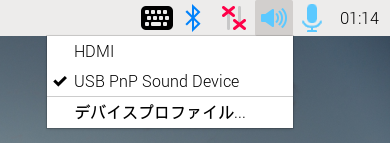
\includegraphics[width=\linewidth]{../../asset/image/pplug-volume_speaker_context_menu.png}
            \caption{USB PnP Sound Device にチェックを入れてしまったら、まずスピーカーアイコンを右クリック。}
            \label{pplug-volume_speaker_context_menu}
        \end{center}
    \end{figure}
\end{minipage}
\begin{minipage}[ht]{0.23\linewidth}
    \begin{figure}[H]
        \begin{center}
            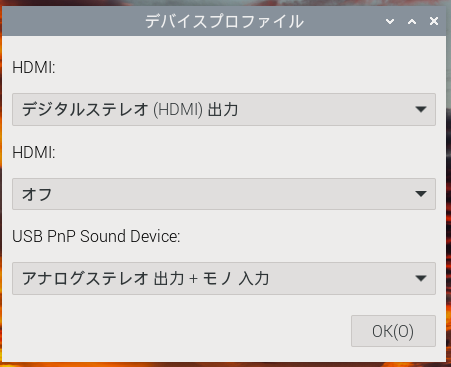
\includegraphics[width=\linewidth]{../../asset/image/pplug-volume_device_profile_top.png}
            \caption{「デバイスプロファイル」ウィンドウを表示}
            \label{pplug-volume_device_profile_dialog_top}
        \end{center}
    \end{figure}
\end{minipage}
\begin{minipage}[ht]{0.23\linewidth}
    \begin{figure}[H]
        \begin{center}
            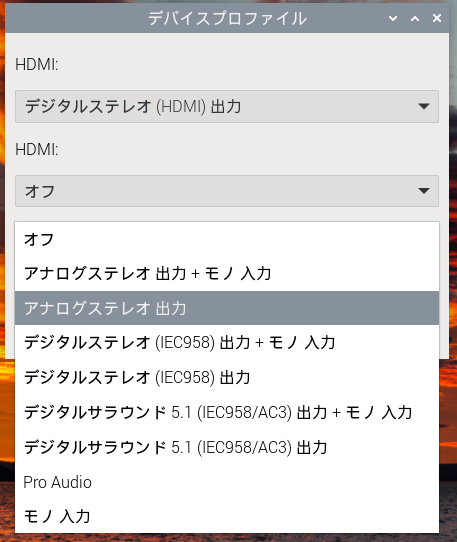
\includegraphics[width=\linewidth]{../../asset/image/pplug-volume_device_profile_dialog_only_output.png}
            \caption{一度「アナログステレオ 出力」を選択。}
            \label{pplug-volume_device_profile_dialog_only_output}
        \end{center}
    \end{figure}
\end{minipage}
\begin{minipage}[ht]{0.23\linewidth}
    \begin{figure}[H]
        \begin{center}
            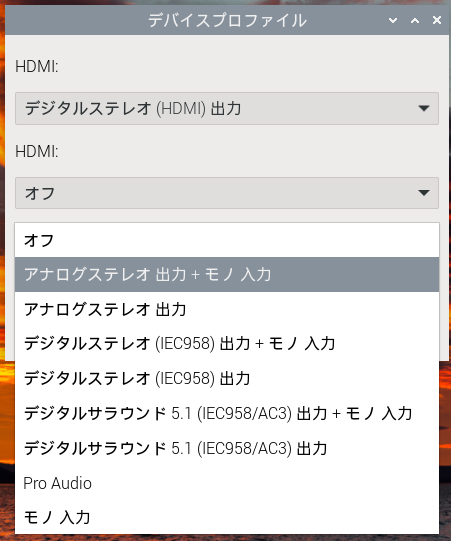
\includegraphics[width=\linewidth]{../../asset/image/pplug-volume_device_profile_dialog_inout.png}
            \caption{「アナログステレオ 出力 + モノ 入力」を選択し、「OK」。}
            \label{pplug-volume_device_profile_dialog_inout}
        \end{center}
    \end{figure}
\end{minipage}
\end{document}
